% ------ headers globales y begin ---------------
\documentclass[11pt, a4paper, twoside]{article}
\usepackage{../header_tp3}
\begin{document}{}
% -----------------------------------------------

Debido a que la soluci\'on exacta es tan costosa de conseguir, contruimos un algoritmo goloso que toma una funci\'on objetivo $f: E  \mapsto \mathbb{R}_+$ para hayar la soluci\'on. La idea de esto es obtener una soluci\'on aproximada en tiempo polinomial. Analizaremos el uso de las 3 criterios y evaluaremos cu\'al implementaci\'on consigue soluciones de mejor calidad. 

Ahora consideremos el siguiente pseudoc\'odigo: 

\begin{algorithm}
In: Grafo $G = (V,X)$, nodo inicial $v_0$, ObjectiveFunction $f$ \newline
Out: Arreglo $\pi$ con camino m\'inimo a cada nodo. 
\begin{algorithmic}[1]
\State $\pi(v) = \infty$ \quad $\forall v \in V$
\State $\pi(v_0) = 0$
\State $S = \emptyset$
\For{$i = 1 \dots n-1$}
    \State $v \leftarrow $ nodo de $V\backslash S$ de m\'inimo $\pi$. 
    \For{{\bf each} $w \in V\backslash S$ adyacente a $v$}
      \State $\pi(w) = \min( \pi(w), \pi(v) + f(v,w))$
    \EndFor
    \State $S = S \bigcup \{v\}$
\EndFor
\Return $\pi$
\end{algorithmic}
\end{algorithm}

Este algoritmo es una modificaci\'on de Dijkstra, que en la l\'inea 7, en vez de sumar $\pi(v)$ m\'as el peso de la arista, como es en el algoritmo original, lo hace m\'as el valor de una funci\'on que define el peso de la arista. Esto nos permite mucha flexibilidad a la hora de cambiar la ``decisi\'on golosa'', y elegir un camino m\'inimo diferente a otro usando otro criterio. As\'i las 3 funciones que elegimos para experimentar son: 

\begin{enumerate}
 \item $f(e) = \omega_1(e)$
 \item $f(e) = \omega_2(e)$
 \item $f(e) = \omega_1(e)\omega_2(e)$
\end{enumerate}

% ME FALTA EXPLICAR PORQUE DIJKSTRA VA A FUNCIONAR COMO HEURISTICA GOLOSA. 

%-- Goloso A --
%\subsubsection{Greedy A}\label{subsubsec:greedy-a}
%Dado un grafo G = (V,E), obtenemos el camino que minimice $w_1$ entre u y v. Utilizamos Dijkstra.
%\clearpage

%-- Goloso B --
%\subsubsection{Greedy B}\label{subsubsec:greedy-b}
%Dado un grafo G = (V,E), obtenemos el camino que minimice $w_2$ entre u y v. Utilizamos Dijkstra.
%\clearpage

%-- Goloso C --
%\subsubsection{Greedy C}\label{subsubsec:greedy-c}
%Dado un grafo G = (V,E), obtenemos el camino que minimice $w_1 * w_2$ entre u y v. Utilizamos Dijkstra.

%-- Familias malas --% 
\fixme{ver adonde poner estas cosas}
Goloso A

\begin{figure}[H]
\begin{center}
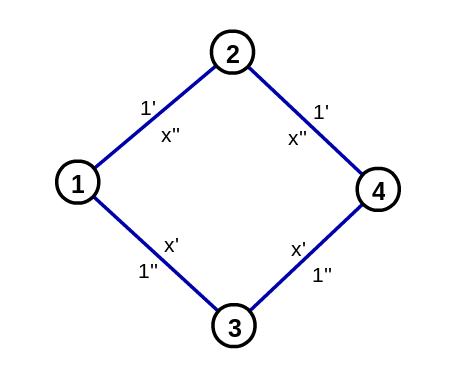
\includegraphics{imagenes/maloGreedyA.png}
\end{center}
\end{figure}

Para ir de 1 a 4 hay dos caminos posibles: (a) 1 -> 2 -> 4 y (b) 1 -> 3 -> 4.
\\sumaOmega1(a) = 2
\\sumaOmega2(a) = 2x
\\sumaOmega1(b) = 2x
\\sumaOmega2(b) = 2

% -----------------------------------------------
\end{document}
